\begin{abstract}
AdaptoFlux is a typed graph substrate for constructing and reusing stateful symbolic programs. It separates editable program graphs from an extensible method pool: declared types guide candidate connections, constructed subgraphs can be registered for subsequent composition, and zero-output action nodes participate in execution without a path to the numerical output. External state connects successive graph executions. Search procedures propose graph structures and method choices; optimized numerical parameters can also be embedded in the resulting programs. Experiments examine semantic type priors, module reuse, execution scale, and integration with an existing graph system. On the studied stateful synthesis task, fine-grained, role-merged, and all-scalar declarations achieve success in 29/30, 15/30, and 1/30 runs. Execution measurements cover up to 1,024 operation nodes. A comparison with PyTensor completes the same discover--register--reuse workflow and reproduces four frozen action controllers over 21,200 steps, with identical actions and zero differences in features, scores, and memory. Controlled search separately identifies benefits of a shared module-reuse policy. An optional resource-ordering mechanism supports consistent shared-state execution. These results characterize concrete interfaces for program modification, reusable computational structure, and stateful interaction.
\end{abstract}

\section{Introduction}
\label{sec:introduction}
Symbolic program synthesis searches over discrete executable structures. Its representation determines which operations can be composed, where intermediate results can be reused, and how a program interacts with mutable state. These choices matter for control tasks: a controller must combine numerical computation with observations, action selection, and environment updates, often over many successive steps. AdaptoFlux makes these interfaces explicit through a typed Method Pool and Generalized Data Flow Graphs (GDFGs).

Consider an action controller that reads an observation $o_t$ and an internal state $h_t$, computes shared features $z_t$, scores each available action, and executes the action selected by an exclusive router. One feature can contribute to several action scores without being recomputed. The state-update branch commits $h_{t+1}$ after reading $h_t$, and the same stored graph runs at the next step. This structure combines typed dataflow, learned numerical parameters, and stateful effects in a single program (Figure~\ref{fig:action_structure}).

\begin{figure}[t]
\centering
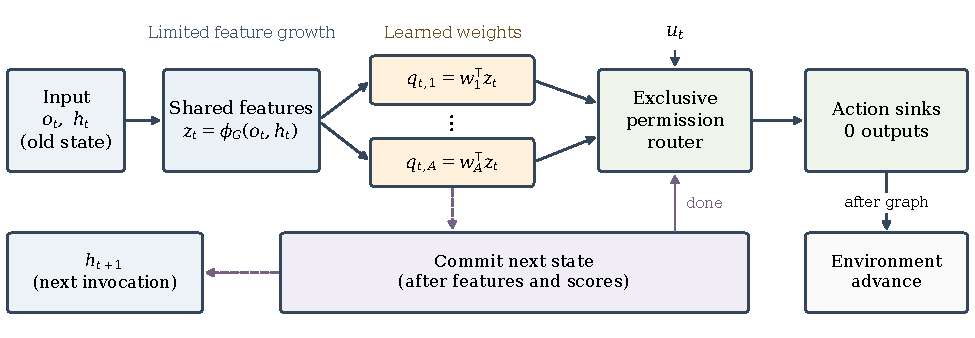
\includegraphics[width=\linewidth]{images/rebuttal_revision/action_structure.pdf}
\caption{A concrete GDFG controller. Shared features feed per-action scores; an exclusive router activates one action. The state branch reads the old state and commits the next state. Dashed purple paths show commit/control relations. The template supplies these interfaces, CMA optimizes score coefficients, and scheduled proposals can extend the feature graph.}
\label{fig:action_structure}
\end{figure}

The representation exposes two objects to learning procedures: a program graph and the method pool from which its nodes are chosen. A graph edit changes a particular program; registering an extracted subgraph expands the vocabulary available to later programs. Declared types constrain candidate connections, and method metadata guides candidate selection. Numerical outputs and environment effects are both observable program behavior: an action branch can matter even when it contributes no returned value. The optional execution contract separately orders conflicting shared-state accesses.

The paper makes three contributions. First, it specifies how typed method declarations, editable graphs, and subgraph registration form a common program-construction interface. Second, it defines execution that includes zero-output actions and repeated interaction with external state; resource-conflict ordering provides an optional consistency extension. Third, controlled studies distinguish the roles of type priors and module reuse, measure execution scale, and compare workflow and action interfaces with an existing graph system. LayerGrow, GraphEvo, and the CMA-based controller optimizer illustrate different procedures operating on these executable structures.

The implementation is available through the anonymous review repository at \url{https://anonymous.4open.science/r/AdaptoFlux-CF54}. Protocols and the provenance of the supplementary measurements are specified in Appendices~\ref{app:revision_effects}--\ref{app:typed_graph_comparisons}.

\section{Positioning and Related Work}
\label{sec:positioning}
Typed program composition, graph reuse, and effect ordering have substantial prior foundations. Strongly typed genetic programming constrains compositions through types~\cite{montana1995strongly}; Cartesian Genetic Programming provides graph-based reuse~\cite{miller2015cartesian}; and MT-CGP explicitly supports mixed data types~\cite{harding2012mtcgp}. LLVM SelectionDAG combines typed dataflow with chain dependencies for side-effect ordering~\cite{llvmSelectionDAG}. These precedents motivate our distinction between data edges and control dependencies.

AdaptoFlux organizes these mechanisms around a method pool and editable program graph. DreamCoder learns reusable abstractions in a functional language~\cite{ellis2021dreamcoder}; Popper uses failure-driven constraint learning~\cite{cropper2021learning}; symbolic-policy and language-model-guided discovery emphasize search quality~\cite{landajuela2021discovering,romera2024mathematical}. PyTensor~\cite{pytensor2026} provides typed computational graphs, native subgraph encapsulation, and Python callbacks. Our comparison identifies concrete interface choices: ATF retains input-ready zero-output actions in graph execution, while the tested PyTensor paths retain effects through requested outputs or shared-variable updates. Both support the tested reuse and action workflows without core changes (Section~\ref{subsec:typed_graph_comparison}). Future work may use language models as candidate generators (Appendix~\ref{app:llm_candidate_generation}). Appendices~\ref{sec:related_work} and~\ref{sec:appendix_baseline_comparison} cover further comparisons, including gplearn and PySR~\cite{cranmer2023interpretable}.

\section{System Architecture}
\begin{figure}[t]
\centering
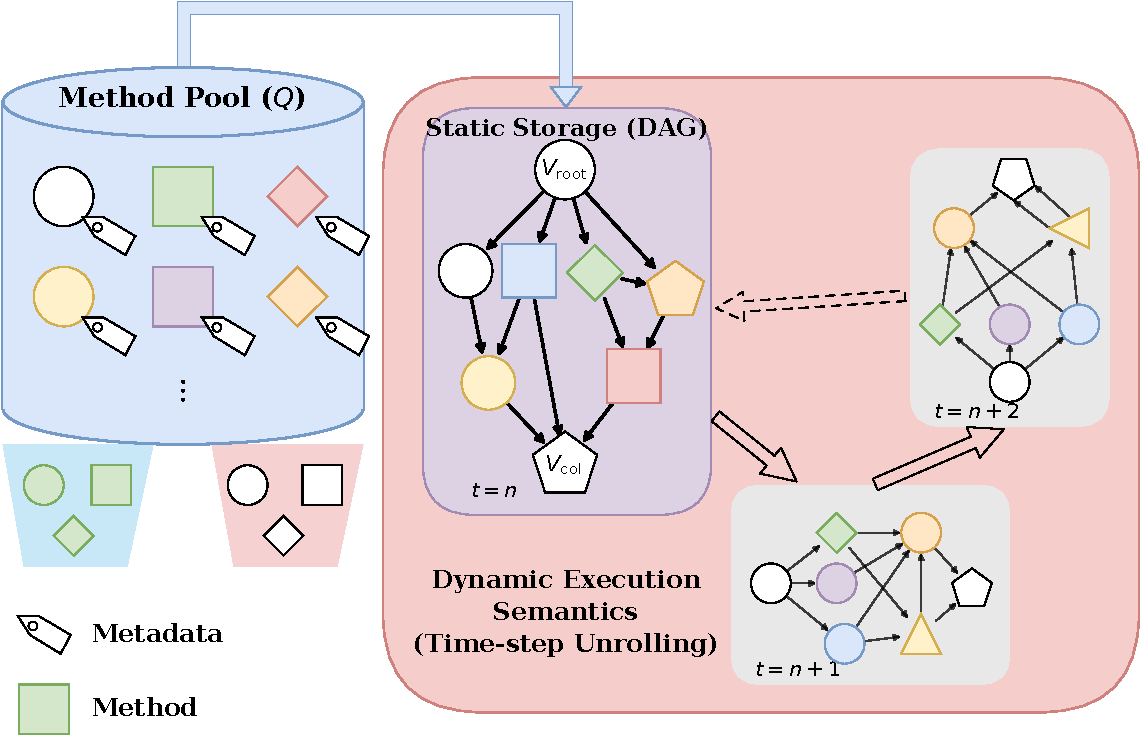
\includegraphics[width=0.74\linewidth]{images/rebuttal_format/NAD.pdf}
\caption{AdaptoFlux architecture. The Method Pool defines callable interfaces, the stored GDFG carries data dependencies, and the runtime connects successive steps through state. Effect-ordering plans add control dependencies to the per-step schedule.}
\label{fig:adaptoflux_arch}
\end{figure}

\subsection{Method Pool}
\label{subsec:method_pool}
A method is registered as $m=\langle\mathrm{impl},\sigma_{\mathrm{in}},\sigma_{\mathrm{out}},\mathrm{M}\rangle$, comprising its implementation, positional input and output type signatures, and metadata. Types are declared atoms, such as \texttt{scalar}, \texttt{pos\_type}, or \texttt{target\_type}. Each input position lists the atoms it accepts; each output port declares the atom it emits. Arity and positional routing determine which outputs can supply which inputs.

Metadata has two roles. Search annotations, including groups and sampling weights, select a view $\mathrm{Q}_{\mathrm{view}}\subseteq\mathrm{Q}$ of the pool. Execution annotations declare the resources a method reads and writes, denoted $R_m$ and $W_m$, or identify a method as pure. Undeclared effects are treated conservatively as unknown. The same resource name must describe accesses to the same external state. A registry entry can also contain a reusable subgraph; its effect contract aggregates those of its constituents. Appendix~\ref{app:metadata_role} separates these execution contracts from search preferences.

\subsection{GDFGs and Stateful Execution}
\label{sec:gdfg}
A data graph $G=\langle V,E_d\rangle$ is a DAG with input, operation, and output-aggregation interfaces. Every operation node is bound to a registered method. An edge connects a particular output port to a particular input position, and is admissible when its emitted type belongs to that position's accepted type set. The data-graph hypothesis class is
\begin{equation}
\label{eq:expression_space}
\Omega_{\mathrm Q,\Sigma}=\{G:\ G\text{ is a DAG},\ m_v\in\mathrm Q,
\text{ and every data edge respects its port types}\}.
\end{equation}
Declared type compatibility is checked during graph construction. The declarations are callable interface contracts: method implementations must also respect their declared inputs and outputs.

\paragraph{Numerical outputs and action execution.}
The runtime executes processing nodes with available inputs, including zero-output action nodes that have no path to the numerical output. The \texttt{collapse} interface collects returned values separately; a valid V0 invocation still requires a connected aggregation interface. An action therefore needs no extra output solely to retain its execution. This rule determines participation in execution, while the ordering contract below determines the order of conflicting state accesses.

\paragraph{State transitions require a selected order.}
For fixed input $x_t$, a node computes data outputs and may update the current external state. Let $\pi=(v_1,\ldots,v_m)$ be a selected topological order. Writing $F_v$ for the state component of node execution, one step is
\begin{equation}
\label{eq:state_transition}
s^{(0)}=s_t,\qquad
s^{(k)}=F_{v_k}(\mathbf{in}_{v_k},s^{(k-1)},x_t),\qquad
s_{t+1}=s^{(m)}.
\end{equation}
The choice of $\pi$ matters. Starting from $s=1$, independent nodes that apply $s\leftarrow s+1$ and $s\leftarrow2s$ produce either $4$ or $3$. Both orders may satisfy the same data DAG. We therefore define the stateful executable program by $P=(G,\pi,E_c)$, where $E_c$ contains control dependencies that preserve the selected order of conflicting accesses.

\paragraph{Optional conflict-aware scheduling.}
Two nodes conflict when
\begin{equation}
W_u\cap(R_v\cup W_v)\ne\varnothing
\quad\text{or}\quad W_v\cap R_u\ne\varnothing.
\end{equation}
For each conflicting pair with $u\prec_\pi v$, the augmented graph $G^+=(V,E_d\cup E_c)$ contains a dependency path from $u$ to $v$. The implementation constructs these paths using resource read/write frontiers; control dependencies carry completion information, while function arguments come only from $E_d$. Shared reads and accesses to disjoint resources remain available for parallel execution. Unknown methods are conservatively ordered with other effectful methods.

With complete effect declarations, deterministic operations, the same inputs and initial state, and successful execution, legal schedules of $G^+$ produce the same outputs and final state. Adjacent independent operations can be exchanged without changing their inputs or resource observations; conflicting operations retain their order. Appendix~\ref{app:revision_effects} gives the execution conditions and validation. If operation-node updates admit increments $I_v$ applied by $\oplus$, and those increments can be evaluated from the same pre-step state and commute on disjoint resources, Equation~\ref{eq:state_transition} reduces to
\begin{equation}
\label{eq:state_parallel}
s_{t+1}=s_t\oplus\bigoplus_{v\in V_{\mathrm{proc}}} I_v(\mathbf{in}_v,s_t,x_t).
\end{equation}

\paragraph{Training and persistence.}
Before a candidate is evaluated, the runtime freezes its initial order. Stable node identities retain that order through accepted substitutions, graph growth, copying, and save/load operations. An explicit order change defines a new candidate for evaluation. For effectful batches, the runtime finishes a complete sample before starting the next. The effect-ordering feature is enabled by default and can be disabled; the selected mode is stored with the model. Disabled mode follows data dependencies and node-wise batching, with no additional state-ordering guarantee.

Across time steps, external state or explicit state inputs connect successive executions of the same stored graph. A finite unrolling uses forward-in-time connections and remains acyclic (Appendix~\ref{app:runtime_loops}). The hand-written Snake example uses mutually exclusive action permits; the controller in Figure~\ref{fig:action_structure} additionally exposes a read-old/commit-new internal-state boundary.

\subsection{Navigation and Reuse}
\label{subsec:navigability_validation}
\textbf{LayerGrow} samples type-compatible operations to extend a graph, evaluates the candidate, and accepts or rolls back the extension. \textbf{GraphEvo} refines a fixed graph skeleton by replacing its bound methods, and can extract subgraphs into reusable methods. With effect ordering enabled, extracted methods retain their internal order and resource declarations; fragments interleaved with external effectful nodes are rejected (Appendix~\ref{app:revision_effects}). \textbf{CombinedTrainer} composes growth and refinement with pool filtering. Their algorithmic descriptions and original experiments are retained in Appendices~\ref{sec:detailed_analysis} and~\ref{sec:appendix_experiments}. The action-controller study uses CMA to optimize numerical score coefficients and scheduled proposals to grow arithmetic features, illustrating a second optimization interface on the same form of executable structure.

\subsection{Execution Cost and Parallelism}
\label{subsec:inference_complexity}
For $V$ operations, $E_d$ data edges, $E_c$ control edges, batch size $N$, and average operation cost $\bar C_{\mathrm{op}}$, inference separates plan preparation, scheduling, routing, and computation:
\begin{equation}
T_{\mathrm{infer}}=T_{\mathrm{prepare}}+T_{\mathrm{sched}}(N,G^+)
+O\bigl(N(|E_d|C_{\mathrm{route}}+V\bar C_{\mathrm{op}})\bigr).
\end{equation}
The revised runtime validates the graph and reconstructs its plan on each call. Pure graphs use one batched traversal, whereas effect-ordered stateful batches use $N$ complete traversals. The threaded implementation sorts ready nodes and creates a worker pool for each traversal; these costs belong to $T_{\mathrm{sched}}$. Resource declarations and the selected ordering determine preparation and control bookkeeping. The historical backend's measurements and complexity breakdown are given in Appendix~\ref{sec:complexity_analysis}.

Parallel benefit depends on the ready graph width, critical path, operation cost, and backend. The original simulated non-blocking workload achieved a mean $10.25\times$ speedup with 16 workers. The supplementary Python scalar CPU workload instead runs faster serially (Section~\ref{subsec:execution_scaling}). Reporting both regimes distinguishes available graph concurrency from the cost of realizing it.

\subsection{Search-Space Structure}
\label{subsec:search_complexity}
Type routing removes inadmissible port compositions before evaluation. Search annotations then select among admissible candidates; effect contracts determine their execution. Increasing the pool can introduce useful operations and simultaneously increase the choices explored under a fixed budget. LayerGrow's cost accumulates across repeated graph extensions, while GraphEvo refinement holds the skeleton fixed. The experiments below measure these effects separately from execution scalability.

\section{Experimental Results}
\label{sec:experiments}
We report three evidence groups: the original navigation experiments, supplementary controlled measurements, and applications developed with additional optimizers. The four supplementary studies of type priors, state encoding, execution scaling, and controller replay used the original frozen ATF backend. The revised effect-aware runtime has a separate regression suite and frozen-model replay audit. Appendix~\ref{app:revision_effects} records this version separation.

\subsection{Structural Search with LayerGrow}
\label{subsec:layergrow_validation}
On Titanic~\cite{titanic}, LayerGrow uses nine scalar operations and a 2,500-attempt budget per run. Across ten runs per maximum-layer setting, mean best accuracy reaches $0.763\pm0.041$ at a configured maximum of 20 layers. Higher requested maxima produce little further improvement (means 0.769--0.783 for settings 25--50) and more budget exhaustion. At requested maxima 45 and 50, all runs exhaust the attempt budget; the mean reached depths are 19.6 and 18.7. Thus the observed failure concerns this growth procedure's progress under its budget. Figure~\ref{fig:scaling_behavior} and Appendix~\ref{sec:appendix_exp1} give the full depth and cost results.

\subsection{GraphEvo and Reusable Subgraphs}
\label{subsec:graphevo_validation}
The task chain is $f_1(x)=2(x+1)$, $f_2(x)=f_1(x)+3$, and $f_3(x)=0.5f_2(x)$. With two-layer initialization for Tasks~1/2, extracted methods yield Task~3 success in 13/100 runs, compared with 0/100 without extraction and 12/100 with a supplied prior. Task~3 always permits at most three top-level calls. Exact enumeration shows that the fixed primitive pools require four calls to express $x+2.5$; composite methods change reachability under that bound. These results measure fixed-depth abstraction (Appendix~\ref{sec:appendix_exp2}).

A separate capacity-matched study gives ATF and an independently implemented reference DAG the same searcher, eight expanded primitive operations, and 256 evaluations per stage. Across 30 seeds per condition, growing versus fixed libraries yield final affine success in 10/30 versus 2/30 runs in both backends, with identical paired search traces. The benefit belongs to the shared module-admission policy; complete results and costs are in Appendix~\ref{app:typed_graph_comparisons}.

\subsection{Semantic Type Priors in Stateful Synthesis}
\label{subsec:stateful_synthesis}
The supplementary Minimal Stateful Attractor experiment holds nine operator implementations fixed and varies only their declared types. The conditions distinguish position and target roles, merge them into one quantity type, or represent all values as scalars. Each condition uses the same 30 search seeds. Each evaluation exhaustively tests the 20 unequal start/target pairs in $\{-2,-1,0,1,2\}$, with at most four graph steps per episode. Strict run success requires solving all 20 pairs.

\begin{table}[t]
\centering
\caption{Semantic type priors improve stateful synthesis. All conditions use the same nine operator bodies and nominal search caps. Evaluation calls report the realized cost; intervals are Wilson 95\% intervals across 30 runs.}
\label{tab:revision_type_main}
\small
\begin{tabular}{lrrr}
\toprule
Type declarations & Successful runs & 95\% interval & Mean calls \\
\midrule
Position / target & 29/30 (96.7\%) & 83.3--99.4\% & 59.47 \\
Merged quantity & 15/30 (50.0\%) & 33.2--66.8\% & 81.67 \\
All scalar & 1/30 (3.3\%) & 0.6--16.7\% & 738.67 \\
\bottomrule
\end{tabular}
\end{table}

Table~\ref{tab:revision_type_main} shows a clear contribution from semantic role information: merging position and target types reduces success from 29 to 15 runs, and flattening all types reduces it to one. Initialization already solves 20, 4, and 0 runs, respectively; refinement supplies the remaining successes. Type declarations improve both the initial candidate distribution and the set of permitted replacements. The realized evaluation budgets differ because stopping conditions and available replacements differ. Appendix~\ref{app:revision_types} reports these budgets, seed-level outcomes, and final-model audits. The original 10-seed experiment, which used a different evaluation protocol and obtained 8/10 versus 0/10, is retained separately in Appendix~\ref{sec:appendix_exp4}.

\subsection{Execution Consistency under Alternative Schedules}
\label{subsec:execution_consistency}
The optional effect-ordering executor preserves a candidate's selected access order through acceptance, copying, and reloads. Replaying 90 frozen models on all 20 initial conditions in serial and three-worker modes matches every trajectory and saved metric: 1,800 model--initial-state pairs and 4,934 paired steps. A six-operation mixed-resource graph agrees under every legal schedule, while a barrier test confirms concurrent execution of independent branches. Targeted tests cover conflicting writes, shared reads, unknown effects, graph edits, and persistence; the recorded regression suite passes 85 tests and 46 subtests. Appendix~\ref{app:revision_effects} gives the execution conditions and complete validation separately from V0 measurements.

\subsection{Implicit and Explicit State Encodings}
For 1,007 candidate/final-model records, implicit accesses are translated into immutable state inputs and outputs while preserving access order. All node values, states, trajectories, and final metrics match across 20,140 paired initial conditions and 70,670 steps. Explicit encoding adds no operation nodes and a mean of 2.189 state edges over the 90 final graphs; its paired execution-time ratio has median 1.137, including state construction and dispatch. Altering the unrelated global state during explicit execution leaves its results unchanged. This measures execution correspondence for already selected programs. Appendix~\ref{app:revision_encoding} gives the translation and timing protocol.

\subsection{Scaling Graphs, Pools, and Execution Workloads}
\label{subsec:execution_scaling}
\paragraph{Single-graph execution.}
At fixed depth eight and batch size 32, we vary width to obtain 32--1,024 operation nodes and 68--2,176 edges, with five graph seeds at each size. Serial time increases from 2.127 to 70.586\,ms across this 32-fold node increase. At the largest size, a separate declared-type compatibility pass takes 1.448\,ms and topological preparation takes 2.310\,ms. Four-worker time is 82.379\,ms: threading is slower for these Python scalar CPU operations. All 30 graphs agree with an independent numerical reference (maximum absolute error $2.22\times10^{-16}$). Figure~\ref{fig:revision_scaling} shows the measured curves; 1,024 nodes is the largest tested point, and the overhead-dominance threshold has not been reached in this sweep.

\begin{figure}[t]
\centering
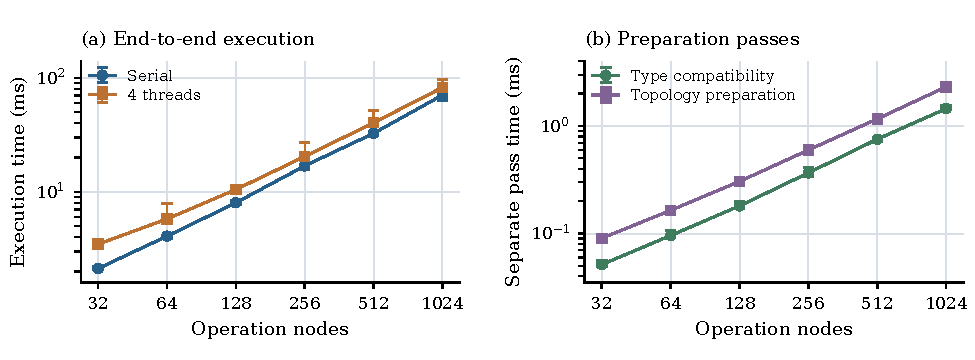
\includegraphics[width=\linewidth]{images/rebuttal_revision/execution_scaling.pdf}
\caption{Fixed-depth scaling on the original backend. Medians summarize five graph seeds per size; error bars show their minimum--maximum range. Each metric uses two warm-ups and seven repetitions. The declared-type pass and topology preparation are measured separately; inference includes its own preparation. Full measurements are in Appendix~\ref{app:revision_scaling}.}
\label{fig:revision_scaling}
\end{figure}

\paragraph{Atomic operator-pool expansion.}
A follow-on search implementation compares nine pools containing 6--20 operators across 12 numerical tasks and four action tasks. Pool expansion has a non-monotonic effect under fixed candidate and interaction budgets (Table~\ref{tab:pool_expansion_main}). The six-operation arithmetic core gives the strongest aggregate numerical pass rate along the nested expansion; adding increment, decrement, and negation gives the strongest maze result. The different responses show that useful operator coverage and the distribution of candidates jointly shape search quality.

\begin{table}[tb]
\centering\small
\caption{Nested atomic-pool expansion. Numerical pass rate averages ten task families and four seeds; maze completion averages two seeds. Both values are percentages.}
\label{tab:pool_expansion_main}
\begin{tabular}{rrr}
\toprule
Operators & Numerical input pass rate & Maze completion \\
\midrule
6 & 14.01 & 11.43 \\
9 & 11.45 & 58.01 \\
15 & 7.72 & 37.89 \\
20 & 11.35 & 6.93 \\
\bottomrule
\end{tabular}
\end{table}

Numerical conditions use 131,072 training input presentations per task and seed, 256 candidate opportunities, and a 32-node graph cap. Action conditions use 65,536 training episodes, 128 candidate opportunities, and a 24-node cap. Numerical success in the table is the fraction of test inputs with relative error at most 1\%. The extensions change operator composition and arity along with pool size. Appendix~\ref{app:revision_pool} gives the full nine-pool comparison and the path-feedback procedure. This experiment identifies a practical design choice: pool views should expose operations relevant to the task while controlling the alternatives presented to a finite-budget optimizer.

\paragraph{Sustained execution and reusable libraries.}
A continual-learning application runs 80 sequences of 40 stages across ten training seeds. Each observation has 64 fields, one of 32 identities, and six available actions. The sequence presents 20 rule families and then returns to them in reverse order. The completed runs record 9,830,400 valid training actions and 229,376,000 evaluation input rows: 239,206,400 input rows in total undergo native-ATF risk-output checks. These counts measure application workload; graph calls can process whole arrays.

\begin{table}[tb]
\centering\small
\caption{Library capacity in the 40-stage application. Costs count environment interactions and average ten paired seeds; lower is better. Return cost measures recovery of previously encountered rule families.}
\label{tab:library_main}
\begin{tabular}{lrrr}
\toprule
Configuration & Capacity & Mean attainment cost & Return cost \\
\midrule
Direct reuse & 32 & 1,792.32 & 1,749.76 \\
Direct reuse & 128 & 1,691.52 & 1,512.96 \\
Full combination & 32 & 1,855.04 & 1,802.88 \\
Full combination & 128 & 1,683.20 & 1,472.00 \\
\bottomrule
\end{tabular}
\end{table}

Attainment cost counts interactions up to the earliest checkpoint after which balanced risk accuracy of at least 90\% and optimal-action rate of at least 80\% in the carrying condition are maintained. A stage that never attains this criterion receives a cost of 3,200. Increasing capacity from 32 to 128 lowers mean attainment cost by 5.62\% for direct reuse and 9.26\% for the full configuration (Table~\ref{tab:library_main}). The full configuration's return cost decreases by 18.35\%, while its first-exposure cost changes little. Additional retained structures therefore help most when earlier tasks are revisited. At capacity 32, the full configuration does not meet its predeclared advantage criterion over direct reuse. A separate shorter capacity sweep shows no stable gain; its capacity-32 and capacity-64 runs produce identical trajectories because occupancy never exceeds 21 entries. The results distinguish retention capacity from the search and selection mechanism used with it. Appendices~\ref{app:revision_large} and~\ref{app:revision_capacity} provide all eight conditions and the short-sequence comparison.

\subsection{A Learned Action-Scoring Controller}
The structure in Figure~\ref{fig:action_structure} computes
\begin{equation}
z_t=\phi_G(o_t,h_t),\qquad q_{t,a}=\sum_j w_{a,j}z_{t,j},\qquad
a_t=\operatorname{route}(q_t,u_t).
\end{equation}
The router uses a supplied draw $u_t$ when its selection rule is stochastic. The template supplies shared features, per-action score branches, exclusive permits, zero-output action sinks, and state-update interfaces. CMA learns the score coefficients; scheduled structure proposals can add arithmetic features or change state-emission sources. Table~\ref{tab:action_main} reports held-out completion across five training seeds, with a separate model for each task.

\begin{table}[tb]
\centering\small
\caption{Held-out action-task completion (\%). Each trained model is evaluated on 2,048 episodes. Mean and range summarize five training seeds; individual results are in Appendix~\ref{app:revision_action}.}
\label{tab:action_main}
\begin{tabular}{llrrr}
\toprule
Task & Completion criterion & Step cap & Mean & Seed range \\
\midrule
Catch & Catch all 16 balls & 160 & 92.10 & 61.28--100.00 \\
Maze & Reach $(7,7)$ & 1,024 & 92.74 & 75.98--98.88 \\
Snake & Collect 8 food items & 512 & 43.55 & 0.05--93.12 \\
Bird & Pass all 32 pipes & 1,024 & 100.00 & 100.00--100.00 \\
\bottomrule
\end{tabular}
\end{table}

Bird succeeds consistently, while Snake exposes substantial training-seed variation. In the validation-selected representative system, Catch, Maze, and Snake have no subsequent feature-growth event; Bird has four. Its 44 shared features supply 88 coefficients. For example, $z_{16}=\texttt{gapBottom}+h^{\mathrm{old}}_1$ enters the flap and coast scores with weights approximately $+3.001$ and $-6.538$, directly illustrating how one state-dependent calculation serves competing action branches. Feature proposals occur at fixed training-budget milestones, so the contribution of optimized coefficients and the occurrence of structural growth can be inspected separately in the saved controller.

A frozen bird model selected by validation was adapted from 314 nodes/411 edges to 316 nodes/565 edges by making its input, state-commit, routing, and observation interfaces explicit. Running this adapted graph in the original ATF executor matches the source controller and an independent interpreter for 20,480 steps over 20 fixed test episodes, with zero difference in features, scores, state, and actions. The replay connects the learned controller to the original execution interface. Appendix~\ref{app:revision_action} gives the five-seed results and adapter specification.

The adapter exposes a complete control step: feature and score nodes read the old state; a single commit node writes the next state; a completion dependency releases the router; the selected action sink records the action; and the environment advances after graph execution. Thus shared computation, state update, and action emission each have an explicit place in the program. The example shows how the representation carries a learned numerical controller while preserving its discrete execution structure.

\subsection{Comparison with a Typed Computational-Graph System}
\label{subsec:typed_graph_comparison}
We implement the same discover--register--reuse workflow in frozen ATF V0 and PyTensor~3.3.8. Each backend evaluates its own candidates and wraps successful programs using \texttt{EvolvedMethod} or \texttt{OpFromGraph}. Twelve method-order cases (11 distinct permutations) produce 36 paired stages and 2,638 candidate evaluations with matching traces. Both systems reuse nested modules and reconstruct programs from common JSON declarations without core changes. Search, admission, and declaration persistence belong to the shared outer procedure.

Four frozen controllers are also expressed through native numerical nodes in both backends. Actions, environment states, features, scores, and memory agree over 21,200 steps; the maximum numerical difference is zero (Table~\ref{tab:typed_graph_interfaces}). Bird additionally matches the existing 20,480-step archive. This is execution migration, with no controller retraining.

\begin{table}[tb]
\centering\small
\caption{ATF V0 and PyTensor interface checks. Controller episodes are fixed evaluation-stream prefixes; counts are coverage, not independent training trials.}
\label{tab:typed_graph_interfaces}
\begin{tabular}{lrl}
\toprule
Check & Paired coverage & Result \\
\midrule
Numerical reuse workflow & 36 stages & Identical traces \\
Catch / Maze / Snake & 720 steps & Identical behavior \\
Bird & 20,480 steps & Identical behavior \\
Routing and state boundaries & 49 cases & All matched \\
\bottomrule
\end{tabular}
\end{table}

The action interface differs in how effects remain executable. ATF retains input-ready zero-output sinks; PyTensor retains the tested callbacks through requested outputs or shared-variable updates. Both mutate the same small environment correctly. PyTensor's \texttt{wrap\_py} decorator also passes this test without handwritten operator classes, with either no optimization or \texttt{FAST\_RUN}; updates allow empty user-visible outputs. Unanchored callback branches are not executed. This distinguishes execution conventions, while ordering conflicting actions remains a separate requirement. Appendix~\ref{app:typed_graph_comparisons} records protocols, native interface boundaries, and the separate reference-DAG search control.

\section*{Limitations}
\label{sec:limitations}
The stateful synthesis task isolates a supplied semantic type prior in a small environment. A remaining comparison is independent search with an explicit-state GP/CGP system under matched realized budgets. The larger applications use additional optimizers and task templates, and their performance depends on these choices. Effect ordering relies on accurate resource declarations; arbitrary Python side effects and runtime exceptions are outside static type compatibility. New-runtime preparation overhead requires its own performance measurements. The graph sweep has not located the practical upper bound or independently varied edge density. Python CPU threading is slower in the measured scalar workload, while the restricted static symbolic-regression benchmark favors specialized solvers on several formulas. These findings identify concrete next steps in search, backend engineering, and evaluation.

\section{Conclusion}
\label{sec:conclusion}
AdaptoFlux organizes editable program graphs, an extensible method pool, and stateful execution through common interfaces. Declared types participate in construction, extracted subgraphs become reusable methods, and zero-output actions participate directly in graph execution. The experiments distinguish supplied type priors, module-reuse policies, execution costs, and integration choices. The PyTensor comparison demonstrates shared workflow capabilities and a concrete difference in retaining effectful branches. Optional resource ordering supplies a separate consistency contract for conflicting state accesses.

Future work will investigate continually learning agents that combine different relation-discovery procedures through this program and method-library interface. The goal is to retain learned subgraphs with applicability conditions and supporting evidence, and use unexpectedly beneficial outcomes and contradictory feedback to guide exploration and local revision. This aims to support knowledge accumulation and adaptation across changing tasks within bounded memory and computation budgets.
\label{maintext:end}
\clearpage

\subsection*{AI use statement}
AI assistants supported the revision through implementation assistance, supplementary experiment scripting, result checking, literature lookup, English drafting and editing, and figure and layout preparation. Numerical results are derived from saved execution records and analysis scripts. The software checks include matched-state replay, independent numerical references, and regression tests. The authors are responsible for the paper's claims and the verification of AI-assisted material.

\subsection*{Ethics statement}
This work follows the ICLR Code of Ethics. It uses public benchmark data and synthetic tasks, involves no human-subject intervention, and reports no personally identifiable experimental data. Automatically generated programs can invoke external actions; applications should validate registered methods and isolate execution environments. Appendix~\ref{app:broader_impacts} discusses interpretability, misuse, and bias inherited from supplied methods.

\subsection*{Reproducibility statement}
The appendices specify method pools, seeds, evaluation criteria, runtime versions, and measurement protocols. The supplementary type study retains final graphs and complete evaluation traces; the state audit retains paired trajectories; the scaling study retains per-seed repetitions and independent reference checks; and the controller case retains its frozen model and stepwise replay. The original implementation and experiment materials are linked through the anonymous repository. Additional evidence is identified by its protocol and artifact names in Appendices~\ref{app:revision_effects}--\ref{app:typed_graph_comparisons}; its execution records are kept separate from historical experiments. Data-graph type checks, effect-ordering assumptions, and finite-unrolling arguments are specified in Sections~\ref{sec:gdfg}--\ref{subsec:inference_complexity} and Appendix~\ref{app:runtime_loops}.
